\documentclass{standalone}
\usepackage{tikz}
\usepackage{pgfplots}

\begin{document}
	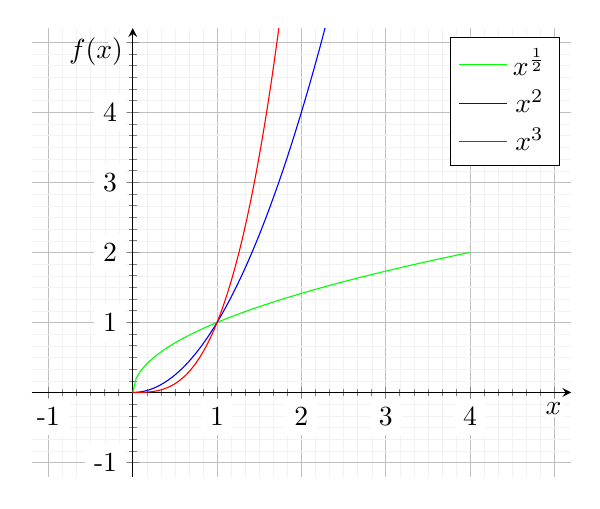
\begin{tikzpicture}
	\begin{axis}[ 
	axis x line = center,
	xlabel = $x$,
	xtick = {-1, 0, 1, 2, 3, 4, 5},
	xticklabels={-1, , 1, 2, 3, 4},
	xlabel style={below left},
	xmin = -1, xmax = 5, 
	axis y line = center,
	ylabel = $f(x)$,
	ylabel style={below left},
	ytick = {-1, 0, 1, 2, 3, 4, 5},
	yticklabels={-1, , 1, 2, 3, 4},
	ymin = -1, ymax = 5,
	ticklabel style={fill=white},
	grid = both,
	enlargelimits={abs=0.2},
	grid style={line width=.1pt, draw=gray!10},
	major grid style={line width=.2pt, draw=gray!50},
	minor tick num=5] 
	\addplot[ domain = 0:4, samples = 100, color = green ] { x^(1/2) };
	\addlegendentry{$x^{\frac{1}{2}}$}
	\addplot[ domain = 0:3, samples = 100, color = blue ] { x^2 };
	\addlegendentry{$x^2$}
	\addplot[ domain = 0:2, samples = 100, color = red ] { x^3 };
	\addlegendentry{$x^3$}
	\end{axis}
	\end{tikzpicture}
\end{document}